\section{Superficies cilíndricas}

\subsection{Definición}

Una superficie cilíndrica en el contexto del cálculo multivariable tiene un significado más general que el cilindro circular de la geometría básica. Engloba cualquier superficie generada por rectas paralelas que barren una curva.

\begin{mydefinition}{Superficie cilíndrica}
Una superficie cilíndrica es una superficie en $\mathbb{R}^3$ formada por todas las rectas generatrices paralelas a un eje fijo y que pasan a través de una curva plana fija denominada curva directriz.
\end{mydefinition}

Ejemplos de identificación:
\begin{itemize}
    \item $x^2 + y^2 = 1$: falta $z$ $\Rightarrow$ cilindro con eje paralelo al eje $z$ (sección circular).
    \item $z = x^2$: falta $y$ $\Rightarrow$ cilindro con eje paralelo al eje $y$ (sección parabólica).
    \item $y^2 - x^2 = 1$: falta $z$ $\Rightarrow$ cilindro con eje paralelo al eje $z$ (sección hiperbólica).
\end{itemize}

\subsection{Cómo graficar una superficie cilíndrica}

\begin{enumerate}
    \item \textbf{Identificar la variable ausente.} Esta indica la dirección de las generatrices.
    \item \textbf{Trazar la curva directriz.} Dibujar la curva en el plano formado por las otras dos variables.
    \item \textbf{Extender.} Extender la curva directriz en ambas direcciones a lo largo del eje de la variable ausente.
\end{enumerate}

\subsubsection{Cilindro circular: $x^2 + y^2 = 1$}

La variable $z$ está ausente. La curva directriz en el plano $xy$ es la circunferencia unitaria. Al extruir a lo largo del eje $z$, obtenemos el cilindro circular recto.

\begin{center}
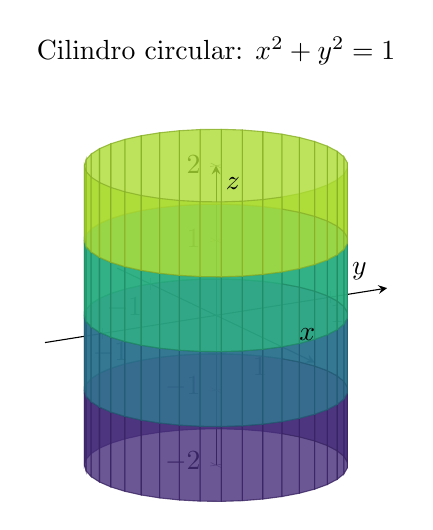
\begin{tikzpicture}
\begin{axis}[
    view={60}{20},
    axis lines=center,
    xlabel=$x$, ylabel=$y$, zlabel=$z$,
    xmin=-1.5, xmax=1.5,
    ymin=-1.5, ymax=1.5,
    zmin=-2, zmax=2,
    colormap/viridis,
    title={Cilindro circular: $x^2 + y^2 = 1$}
]
\addplot3[
    surf,
    parametric,
    domain=0:360,
    domain y=-2:2,
    samples=40,
    samples y=5,
    opacity=0.8
] ({cos(x)}, {sin(x)}, {y});
\end{axis}
\end{tikzpicture}
\end{center}

\subsubsection{Cilindro parabólico: $z = x^2$}

La variable $y$ está ausente. La curva directriz en el plano $xz$ es la parábola $z = x^2$. Al extruir a lo largo del eje $y$, obtenemos el cilindro parabólico.

\begin{center}
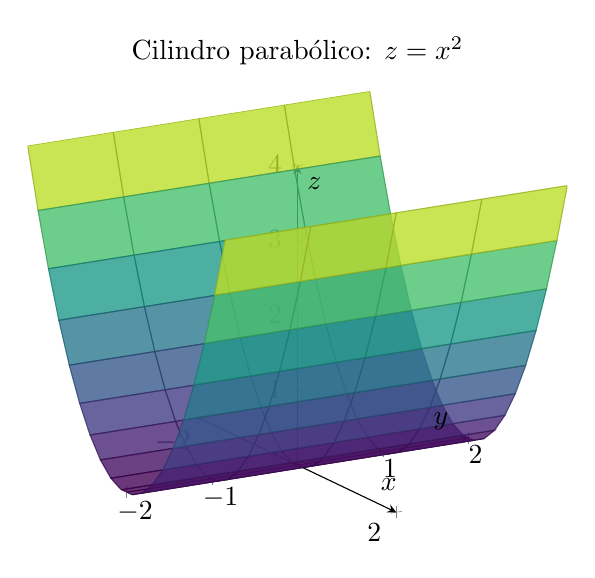
\begin{tikzpicture}
\begin{axis}[
    view={60}{20},
    axis lines=center,
    xlabel=$x$, ylabel=$y$, zlabel=$z$,
    colormap/viridis,
    title={Cilindro parabólico: $z = x^2$}
]
\addplot3[
    surf,
    domain=-2:2,
    domain y=-2:2,
    samples=20,
    samples y=5,
    opacity=0.8
] {x^2};
\end{axis}
\end{tikzpicture}
\end{center}


\subsection{Ejercicios}

\begin{enumerate}
    \item Identificar el tipo de cada superficie cilíndrica, señalar la variable ausente, describir la curva directriz y el eje a lo largo del cual se extiende la superficie.
\begin{enumerate}
    \item $x^2 + z^2 = 9$
    \item $y = \sin(x)$
    \item $4x^2 + 9y^2 = 36$
    \item $z = e^x$
\end{enumerate}
    \item Determinar la ecuación del cilindro cuyas generatrices son paralelas al eje $z$ y cuya curva directriz en el plano $xy$ es la elipse con semiejes $a = 3$ en la dirección $x$ y $b = 2$ en la dirección $y$, centrada en el origen.

Verificar que los puntos $P_1 = (3, 0, 5)$ y $P_2 = (0, 2, -7)$ pertenecen a la superficie, y determinar si $P_3 = (2, 1, 4)$ pertenece o no.
    \item Para el cilindro parabólico $y = x^2 - 4x + 3$:
\begin{enumerate}
    \item Completar el cuadrado para escribir la ecuación en la forma $y = (x - h)^2 + k$ e identificar el vértice de la parábola directriz.
    \item Señalar cuál es la variable ausente y describir el eje del cilindro.
    \item Encontrar la intersección del cilindro con el plano $z = 2$ y con el plano $x = 1$.
    \item Determinar si el punto $Q = (2, -1, 100)$ pertenece al cilindro.
\end{enumerate}
    \item La recta $L: \vec{r}(t) = (1,\, 0,\, -1) + t(0,\, 1,\, 3)$ y el cilindro circular $x^2 + y^2 = 5$.
\begin{enumerate}
    \item Determinar si la recta es paralela, interseca o está contenida en el cilindro.
    \item Si la recta interseca al cilindro, encontrar todos los puntos de intersección.
    \item Encontrar la distancia del eje del cilindro (el eje $z$) a la recta $L$.
\end{enumerate}

\textit{Sugerencia:} Sustituir las expresiones paramétricas de $x$ e $y$ en la ecuación del cilindro y resolver en $t$.
    \item Encontrar la ecuación del cilindro con generatrices paralelas al eje $y$ que contiene a la curva de intersección de las superficies $z = x^2 + 1$ y $z = 4 - x^2$.

\begin{enumerate}
    \item Encontrar las curvas de intersección igualando las dos ecuaciones.
    \item Eliminar la variable $z$ para obtener la ecuación del cilindro en el plano $xy$.
    \item Describir geométricamente la curva directriz obtenida.
\end{enumerate}
    \item Escribir las ecuaciones paramétricas de cada superficie cilíndrica e identificar el rango de los parámetros para cubrir la superficie completa.
\begin{enumerate}
    \item Cilindro circular $x^2 + z^2 = 4$ (eje $y$), para $-3 \leq y \leq 3$.
    \item Cilindro elíptico $\dfrac{x^2}{9} + \dfrac{z^2}{4} = 1$ (eje $y$), para $y \in \mathbb{R}$.
    \item Cilindro parabólico $z = x^2$ (eje $y$), para $-2 \leq x \leq 2$, $-2 \leq y \leq 2$.
\end{enumerate}

\textit{Sugerencia:} Para cónicas en el plano $xz$, usar una parametrización trigonométrica o explícita según corresponda, y agregar $y = t$ como parámetro libre.
    \item Clasificar cada ecuación como cilindro o no. Si es un cilindro, identificar el tipo y la variable ausente. Si no lo es, justificar brevemente.
\begin{enumerate}
    \item $x^2 + y^2 + z^2 = 16$
    \item $x^2 - y^2 = 1$
    \item $z = \ln(x^2 + 1)$
    \item $xy = 4$
    \item $x^2 + y^2 + z = 0$
    \item $x^2 + z^2 - 4x + 2z - 4 = 0$
\end{enumerate}

Para el inciso (f), completar el cuadrado en las variables correspondientes y escribir la ecuación en forma estándar.
    \item El cilindro hiperbólico $x^2 - y^2 = 1$ tiene generatrices paralelas al eje $z$.
\begin{enumerate}
    \item Identificar los vértices y asíntotas de la hipérbola directriz en el plano $xy$.
    \item Determinar la traza del cilindro con el plano $z = k$ para cualquier valor de $k$.
    \item Encontrar la intersección del cilindro con el plano $y = 2$ y describir qué curva se obtiene.
    \item Verificar que el punto $P = (\sqrt{2},\, 1,\, -3)$ pertenece al cilindro.
    \item Encontrar todos los puntos del cilindro con $x = 2$, $z = 0$.
\end{enumerate}
    \item Determinar la ecuación del cilindro con generatrices paralelas al eje $z$ que pasa por la curva $C$ definida por la intersección de:
\[
x^2 + y^2 + z^2 = 9 \quad \text{y} \quad z = 1
\]

\begin{enumerate}
    \item Encontrar la curva $C$ sustituyendo $z = 1$ en la ecuación de la esfera.
    \item Eliminar la variable $z$ para obtener la ecuación del cilindro proyectado sobre el plano $xy$.
    \item Describir geométricamente la superficie cilíndrica obtenida e indicar su radio.
    \item Encontrar la intersección del cilindro obtenido con el plano $y = 0$.
\end{enumerate}
    \item La región sólida $E$ está acotada por el cilindro circular $x^2 + y^2 = 4$, el plano $z = 0$ y el plano $z = 3$.
\begin{enumerate}
    \item Describir en palabras la forma del sólido $E$.
    \item Determinar si el punto $Q = (1,\, 1,\, 2)$ está dentro, fuera o sobre la frontera de $E$.
    \item Encontrar la longitud del segmento de la recta $\vec{r}(t) = (1,\, 0,\, t)$, $t \in \mathbb{R}$, que se encuentra dentro de $E$.
    \item Dos cilindros, $x^2 + y^2 = 4$ y $x^2 + z^2 = 4$, se intersectan. Encontrar y describir la curva de intersección en la región $x \geq 0$.

    \textit{Sugerencia:} En la curva de intersección se cumple $y^2 = z^2$; usar esto para parametrizar.
\end{enumerate}
\end{enumerate}
